\section{Definitions}

\paragraph{Solipsis Objects}
The \sol metaverse consists of a set of \emph{entities}, each
belonging to one of three categories: \emph{avatars}, \emph{objects},
and \emph{sites}. Avatars are the main actors of the metaverse as they
are the only entities that are capable of autonomous movement. In most
cases they are virtual representations of the users of the metaverse
and are directly controlled by them using the navigator platform.
Objects, on the other hand, are virtual representation of entities
from the real world such as furniture, books and whatever object may
be moved or picked up by an avatar. Avatar and objects may also be
robotic-like entities controlled by user-defined software
components. Finally, sites constitute the basic building blocks of the
metaverse and represents portions of the virtual space that may be
occupied by objects or in which avatars can roam.


Avatars, objects, and sites are all associated with 3D-descriptions,
which constitute the basis for the rendering of entities in the
navigator platform. The 3D description of an entity contains all the
information necessary for its 3D visualization: this includes a mesh-
or prims-based model, a set of textures, and, in the case of avatars
or objects, an animation. In addition the 3D-description may contain
sounds, videos, or multimedia content associated with the entity. From
the point of view of this protocol, such a representation merely
consists of a set of binary objects, or files, that should be provided
to the rendering component. Each such object is associated with its
own version number and may thus be updated independently of the
others.

% From the point of view of this specification,
% each component of a 3D-description is represented by a file that can
% be downloaded from a remote host, stored locally, and offered for
% download to other hosts in the network. 

% Nonetheless, the protocol can
% easily support several levels of details with only minor
% modifications. The two levels we consider consist of a \emph{complete
%   description} of the object and of a an% \df{This will change. Ultimately we are going to have:
%   descriptor, and 3dData, which in turn consists of mesh, texture, and
%   animation.}.

The state of an entity in the metaverse is determined by an
\emph{entity descriptor}, from now on referred to simply as
\emph{descriptor}.  An entity's descriptor consist of the minimal
information required to display a rough representation of the entity
and includes, for example, the its location, its shape, its size, and its
orientation.

% , and its visibility radius, vRadius. The shape of the
% object is represented by an identifier that selects one from a set of
% predefined shapes; while its visibility radius identifies the distance
% from which the object should be visible in the absence of obstacles
% and without any visual aids.

% An entity's descriptor can contains information
% regarding its position, its physical properties, and whatever is
% needed to display the entity and compute its interaction with the rest
% of the metaverse. For example, a descriptor containing a key frame can
% be used to synchronize animations, and videos. %  Moreover, it may
% contain 
% filtering descriptors defining areas (concentric spheres, hierarchical
% partitioning, cells) associated with a level of detail or a set of
% visible objects may be used to achieve efficient on-demand streaming
% while satisfying view-dependency criteria. Finally, descriptors may
% contain load-balancing information regarding, for example, the
% available resources or serving capabilities of a
% host~\cite{cavagna}.
% % auto-regulate the network load
% Table~\ref{tab:desc} shows a sample descriptor containing the
% most relevant information. Although the descriptor is shown as a
% single object, the \sol implementation may split it into several
% descriptors regarding, for example, physical properties,
% location, or level of details in order to reduce communication cost.


Descriptors also keep track of which hosts have recorded a copy of the
corresponding entity's 3D description. Specifically, each descriptor
contains two fields associated with each of the files that constitute
the a 3D description. The first field is the latest known version
number of the file, while the second is a list of hosts that are known
to have cached a copy of the version of the file indicated in the
first field.

The descriptor is the means through which the \sol protocol tracks the
evolution of an entity. To maintain consistency, each descriptor is
associated with a sequence number that is incremented each time the
descriptor is modified. A minimal descriptor is shown in
Table~\ref{tab:desc}. 

% The general rule for modifying object
% descriptors in the \sol protocol is that each descriptor may be
% modified only by the site node that is responsible for the current
% location of the corresponding object. This is straightforward in the
% case of static objects (sites), but is somewhat more complex in the
% case of roaming objects (avatars), as these may roam move from one
% location to another and thus from one site node to another.


% %THIS SHOULD PROBABLY BE BROUGHT BACK
% Specifically, in the case of roaming object, the node responsible for
% the object's location may not be the same as the node that is
% currently owning the object. Yet, the owner of the object should still
% be entitled to modify attributes of the object descriptor such as the
% shape or the files associated with the 3D model. Details about how
% this is achieved are given in Section~\ref{}. 


%  o make this
% possible, we also define for roaming objects, an additional
% \emph{static descriptor}\df{need a better name}, which includes all
% the fields in the object descriptors excluding location and
% orientation. The static descriptor of a roaming object can only be
% modified by the owner of the object, while the object descriptor is
% managed by the node responsible for the object location, as described
% in Section~\ref{}. 

% Finally, in future versions of the protocol, the object descriptor may
% contain information required to implement progressive levels of
% details in the 3D representations of objects.  A summary of the fields
% included in an object descriptor is shown in Table~\ref{tab:desc}.

\begin{table}
\centering
\begin{tabular}{|l|p{8cm}|}
\hline
  $\mathsf{UID}$ & universal identifier of the entity\\
  $\mathsf{seqNum}$ & sequence number\\
\hline
  $\mathsf{owner}$ & identifier of the node managing the entity\\
  $\mathsf{type}$ & site or avatar\\
  $\mathsf{loc}$ & location in the 3D space\\
  $\mathsf{ori}$ & orientation in the 3D space\\
  $\mathsf{shape}$& shape from a predefined set\\
  $\mathsf{box}$ & bounding box of the object\\
  $R_p$ & perceptibility radius: distance from which the object is
  visible in the absence of obstacles\\
  $R_b$ & radius of  smallest sphere enclosing the entity\\
  $\mathsf{objs}_a$ & list of entities attached to the current one\\
  \hline
  $f_1$ & first file of 3d-description \\
  $v_1$ & version number for first file\\
  $c_1$ & list of hosts that have cached $v_1$ of $f_1$\\
  ...& ...\\
  $f_n$& n-th file of 3d-description\\
  $v_n$& version number for n-th file\\
  $c_n$& list of hosts that have cached $v_n$ of $f_n$\\
  \hline
  ... & additional fields for progressive levels of details\\
  \hline
\end{tabular}

\caption{Format of an object descriptor}
\label{tab:desc}
\end{table}


\subsection{Solipsis Hosts and Nodes}
From a practical viewpoint, the \sol platform is distributed over a
set of \emph{hosts}, also referred to as \emph{peers} that maintain
information about every entity that is currently present in the
metaverse.  Each host is associated with a single instance of the \sol
platform, and throughout its lifetime, it may create new entities or
destroy previously created ones according to the requests of the
navigator component. Also, similar to an entity, each host is
associated with a unique identifier (UID).

Because each host may be responsible for several entities at the same
time, we define a \emph{(Solipsis) node} as the set of resources
dedicated to the management of a given entity. Each node incapsulates
information about the corresponding entity's descriptors as well as
the threads of control responsible for managing all the interactions
of the node with the rest of the \sol metaverse as well as with the
navigator platform. Depending on the type of entity they are managing,
we distinguish three types of \sol nodes: \emph{site nodes},
\emph{avatar nodes}, and \emph{object nodes}. 




\subsection{P2P Architecture}
Nodes are organized in a three-dimensional overlay network based on
the Raynet protocol. The arrangement of nodes in this overlay is based
on the locations of the corresponding sites in the \sol world. In
particular, each site node is responsible for a section of the world,
its \emph{cell}, centered around its own site and comprising a region
of space around it. This is achieved by subdividing space according to
a Voronoi tessellation, as shown in
Figure~\ref{Fig:Overview}. Neighborhood relationships between peers
are determined by the distance between the corresponding points in
this space. Specifically, two Raynet nodes are neighbors in the
overlay if the two corresponding points are neighbors in the Delaunay
graph comprising all the points associated with Raynet nodes.

\begin{figure}
\center
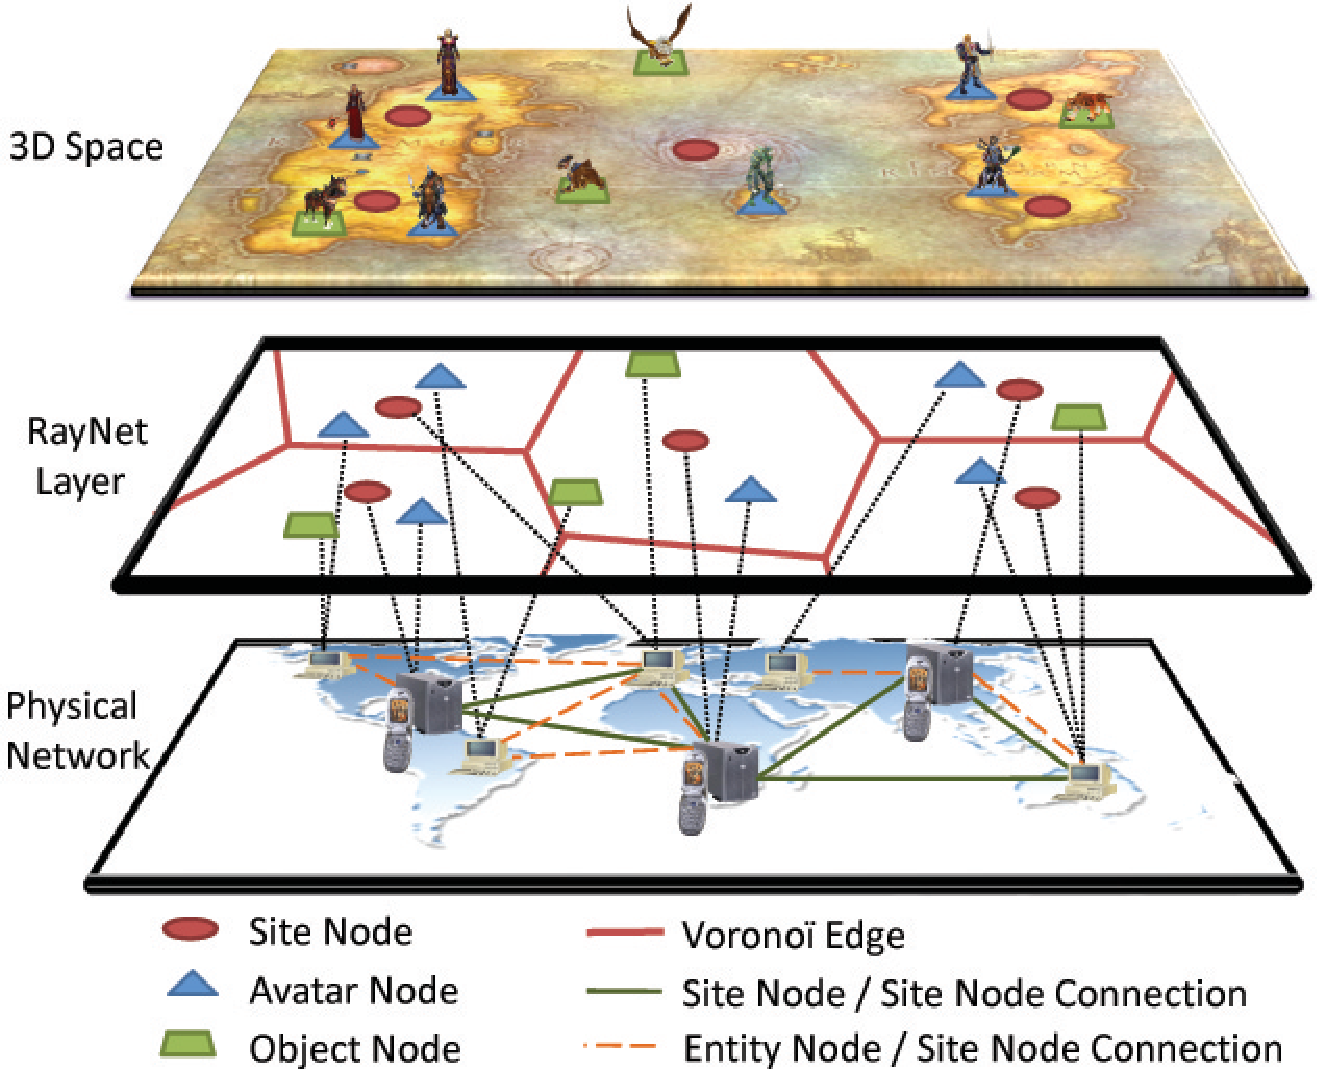
\includegraphics[width=3in]{figs/overview.pdf}
\caption{The p2p architecture showing the mapping of the raynet layer on the virtual world layer according to the proximity of nodes in the virtual space. The host layer shows clients connected into a peer to peer scheme.}
\label{Fig:Overview}
\end{figure}

Given a set of generator points$\{p \in \Re^d\}$, the Delaunay graph
is obtained as the adjacency graph of the corresponding Voronoi
diagram, which in turn is a tessellation of the d-dimensional space
$\Re^d$. Specifically, the cell in the tessellation associated with a
point $p_x$ is such that it contains all the points that are closer to
$p_x$ than to any other generator point in the set.







%%% Local Variables: 
%%% mode: latex
%%% TeX-master: "specification"
%%% End: 
